\documentclass[a4paper,UTF8]{article}
\usepackage{ctex}
\usepackage[margin=1.25in]{geometry}
\usepackage{color}
\usepackage{graphicx}
\usepackage{amssymb}
\usepackage{amsmath}
\usepackage{amsthm}
\usepackage{enumerate}
\usepackage{bm}
\usepackage{hyperref}
\usepackage{epsfig}
\usepackage{color}
\usepackage{mdframed}
\usepackage{lipsum}
\usepackage{graphicx}
\newmdtheoremenv{thm-box}{Theorem}
\newmdtheoremenv{prop-box}{Proposition}
\newmdtheoremenv{def-box}{定义}

\usepackage{listings}
\usepackage{xcolor}
\lstset{
	numbers=left, 
	numberstyle= \tiny, 
	keywordstyle= \color{ blue!70},
	commentstyle= \color{red!50!green!50!blue!50}, 
	frame=shadowbox, % 阴影效果
	rulesepcolor= \color{ red!20!green!20!blue!20} ,
	escapeinside=``, % 英文分号中可写入中文
	xleftmargin=2em,xrightmargin=2em, aboveskip=1em,
	framexleftmargin=2em
} 

\usepackage{booktabs}

\setlength{\evensidemargin}{.25in}
\setlength{\textwidth}{6in}
\setlength{\topmargin}{-0.5in}
\setlength{\topmargin}{-0.5in}
% \setlength{\textheight}{9.5in}
%%%%%%%%%%%%%%%%%%此处用于设置页眉页脚%%%%%%%%%%%%%%%%%%
\usepackage{fancyhdr}                                
\usepackage{lastpage}                                           
\usepackage{layout}                                             
\footskip = 12pt 
\pagestyle{fancy}                    % 设置页眉                 
\lhead{2020年春季}                    
\chead{机器学习导论}                                                
% \rhead{第\thepage/\pageref{LastPage}页} 
\rhead{作业二}                                                                                               
\cfoot{\thepage}                                                
\renewcommand{\headrulewidth}{1pt}  			%页眉线宽,设为0可以去页眉线
\setlength{\skip\footins}{0.5cm}    			%脚注与正文的距离           
\renewcommand{\footrulewidth}{0pt}  			%页脚线宽,设为0可以去页脚线

\makeatletter 									%设置双线页眉                                        
\def\headrule{{\if@fancyplain\let\headrulewidth\plainheadrulewidth\fi%
\hrule\@height 1.0pt \@width\headwidth\vskip1pt	%上面线为1pt粗  
\hrule\@height 0.5pt\@width\headwidth  			%下面0.5pt粗            
\vskip-2\headrulewidth\vskip-1pt}      			%两条线的距离1pt        
 \vspace{6mm}}     								%双线与下面正文之间的垂直间距              
\makeatother  

%%%%%%%%%%%%%%%%%%%%%%%%%%%%%%%%%%%%%%%%%%%%%%
\numberwithin{equation}{section}
%\usepackage[thmmarks, amsmath, thref]{ntheorem}
\newtheorem{theorem}{Theorem}
\newtheorem*{definition}{Definition}
\newtheorem*{solution}{Solution}
\newtheorem*{prove}{Proof}
\newcommand{\indep}{\rotatebox[origin=c]{90}{$\models$}}

\usepackage{multirow}

%--

%--
\begin{document}
\title{机器学习导论\\
作业二}
\author{171830635, 俞星凯, yuxk@smail.nju.edu.cn}
\maketitle

\section{[15 pts] Linear Regression}
给定数据集$D=\{(\mathbf{x}_i,y_i)\}_{i=1}^m$,最小二乘法试图学得一个线性函数$y=\mathbf{w^*}\mathbf{x}+b^*$使得残差的平方和最小化,即
\begin{equation}
	(\mathbf{w^*},b^*) = \mathop{\arg\min}_{\mathbf{w},b} \sum_{i=1}^m [y_i-(\mathbf{w}\mathbf{x_i}+b)]^2 . 
\end{equation}
“最小化残差的平方和”与“最小化数据集到线性模型的欧氏距离之和”或是“最小化数据集到线性模型的欧氏距离的平方和”一致吗?考虑下述例子
\begin{equation}
	D = \{ (-1,0) , (0,0) , (1,1) \} , 
\end{equation}
并回答下列问题。

\begin{enumerate}[(1)]
	\item \textbf{[5 pts]} 给出“最小化残差的平方和”在该例子中的解$(w^*,b^*)$。
	\item \textbf{[5 pts]} 给出“最小化数据集到线性模型的欧氏距离的平方和”在该例子中的数学表达式,并给出其解$(w_{E},b_{E})$,该解与$(w^*,b^*)$一致吗?
	\item \textbf{[5 pts]} 给出“最小化数据集到线性模型的欧氏距离之和”在该例子中
	的数学表达式,$(w^*,b^*)$是该问题的解吗?
\end{enumerate}

\begin{solution}
	此处用于写解答(中英文均可)
	\begin{enumerate}[(1)]
		\item 
		\begin{align*}
		(w^*,b^*)
		&=\mathop{\arg\min}_{w,b}(0+w-b)^2+b^2+(1-w-b)^2\\
		&=\mathop{\arg\min}_{w,b}2w^2-2w+3b^2-2b+1\\
		&=\mathop{\arg\min}_{w,b}2(w-\frac12)^2+3(b-\frac13)^2+\frac16\\
		&=(\frac12,\frac13)
		\end{align*}
		
		\item 
		\begin{equation*}
		(w_E,b_E)=\mathop{\arg\min}_{w,b}\lVert 0+w-b\rVert_2^2+\lVert b\lVert_2^2+\lVert 1-w-b\rVert_2^2
		\end{equation*}
		$(w_E,b_E)$与$(w^*,b^*)$一致。
		
		\item 
		\begin{equation*}
		(w_S,b_S)=\mathop{\arg\min}_{w,b}\lvert0+w-b\rvert+\lvert b\rvert+\lvert1-w-b\rvert
		\end{equation*}
		$(w^*,b^*)$不是该问题的解,因为$(\frac12,\frac12)$是更优解。
		
	\end{enumerate}
\end{solution}

\section{[40+5 pts] 编程题, Logistic Regression}
\textbf{请结合编程题指南进行理解}
\par 试考虑对率回归与线性回归的关系。最简单的对率回归的所要学习的任务仅是根据训练数据学得一个$\beta=(\omega;b)$,而学习$\beta$的方式将有下述两种不同的实现:
\par 0. [闭式解] 直接将分类标记作为回归目标做线性回归,其闭式解为 \begin{equation}
	\beta=({\hat{X}}^T\hat{X})^{-1}\hat{X}^Ty
	\end{equation}, 其中$\hat{X}=(X;\vec{1})$

\par 1. [数值方法] 利用牛顿法或梯度下降法解数值问题
\begin{equation}
	\min_{\mathbf{\beta}} \sum_{i=1}^{m}(-y_i\beta^T\hat{x_i}+\ln (1+e^{\beta^T\hat{x_i}})). 
\end{equation}
得到$\beta$后两个算法的决策过程是一致的,即:
\begin{enumerate}[(1)]
	\item $z=\beta X_{i}$
	\item $f=\frac{1}{1+e^{-z}}$
	\item 决策函数\begin{equation}
		y_{i}=
		\begin{cases}
		1,&\mbox{if $f>\theta$}\\
		0,&\mbox{else}
		\end{cases}
		\end{equation}
	\end{enumerate}
	其中$\theta$为分类阈值。回答下列问题:
	\begin{enumerate}[(1)]
		\item \textbf{[10 pts]} 试实现用闭式解方法训练分类器。若设分类阈值$\theta=0.5$,此分类器在Validation sets下的准确率、查准率、查全率是多少?
		\item \textbf{[10 pts]} 利用所学知识选择合适的分类阈值,并输出闭式解方法训练所得分类器在test sets下的预测结果。
		\item \textbf{[10 pts]} 利用数值方法重新训练一个新的分类器。若设分类阈值$\theta=0.5$,此分类器在Validation sets下的准确率、查准率、查全率是多少?
		\item \textbf{[10 pts]} 利用所学知识选择合适的分类阈值,并输出数值方法训练所得分类器在test sets下的预测结果。
		\item \textbf{[选做][Extra 5 pts]} 谈谈两种方法下分类阈值的变化对预测结果的影响,简要说明看法。
	\end{enumerate}
\begin{solution}
	此处用于写解答(中英文均可)
	\begin{enumerate}[(1)]
		\item 
		准确率0.74,查准率0.67,查全率1.00。
		\item 
		选择$\theta=0.55$,准确率、查准率、查全率都是1.0。
		\item 
		准确率、查准率、查全率都是1.0。
		\item 
		选择$\theta=0.55$,准确率、查准率、查全率仍然都是1.0。
		\item 
		sigmoid函数的图像特点是中间陡峭,两边平缓。因为在$y$方向上变化相同长度时,在$x$方向上的变化两边比中间大,所以当阈值在中间0.5附近变化时,对预测结果影响较小;当阈值在0和1附近变化时,对预测结果影响较大。
	\end{enumerate}
\end{solution}

\section{[10 pts] Linear Discriminant Analysis}
在凸优化中,试考虑两个优化问题,如果第一个优化问题的解可以直接构造出第二个优化问题的解,第二个优化问题的解也可以直接构造出第一个优化问题的解,则我们称两个优化问题是等价的。基于此定义,试证明优化问题\textbf{P1}与优化问题\textbf{P2}是等价的。
\begin{equation}
	\label{P1}
	\max_{\mathbf{w}} \frac{\mathbf{w}^\top S_b \mathbf{w}}{\mathbf{w}^\top S_w \mathbf{w}} . 
\end{equation}
\begin{equation}
	\label{P2}
	\begin{aligned}
		\min_{\mathbf{w}} & \quad -\mathbf{w}^\top S_b \mathbf{w} \\ 
		\text{s.t.} & \quad \mathbf{w}^\top S_w \mathbf{w} = 1 . 
	\end{aligned}
\end{equation}

\begin{solution}
	~\\
	设\textbf{P1}的解$\mathbf{w}$,则$k\mathbf{w}$也是解,令$k=\sqrt{\mathbf{w}^\top S_w \mathbf{w}}$,则$(k\mathbf{w})^\top S_w (k\mathbf{w})=1$,并且$(k\mathbf{w})^\top S_b (k\mathbf{w})$最大,即$-(k\mathbf{w})^\top S_b (k\mathbf{w})$最小,因此$kw$是\textbf{P2}的解。\\
	设\textbf{P2}的解$\mathbf{w}$,则$k\mathbf{w}$是问题\textbf{P3}的解。
	\begin{equation*}
	\begin{aligned}
	\max_{\mathbf{w}} & \quad \frac{\mathbf{w}^\top S_b \mathbf{w}}{\mathbf{w}^\top S_w \mathbf{w}} \\ 
	\text{s.t.} & \quad \mathbf{w}^\top S_w \mathbf{w} = k^2
	\end{aligned}
	\end{equation*}
	因为$k$是任意的,所以去除约束条件,$\mathbf{w}$是\textbf{P1}的解。
\end{solution}
\section{[35 pts] Multiclass Learning}
在处理多分类学习问题的时候,我们通常有两种处理思路:一是间接求解,利用一些基本策略(OvO, OvR, MvM)将多分类问题转换为二分类问题,进而利用二分类学习器进行求解。二是直接求解,将二分类学习器推广到多分类学习器。
\subsection{问题转换}
\begin{enumerate}[(1)]
	\item \textbf{[5 pts]} 考虑如下多分类学习问题:假设样本数量为$n$,类别数量为$C$,二分类器对于大小为$m$的数据训练的时间复杂度为$ \mathcal{O}(m) $(比如利用最小二乘求解的线性模型)时,试分别计算在OvO、OvR策略下训练的总时间复杂度。
	\item \textbf{[10 pts]} 当我们使用MvM处理多分类问题时,正、反类的构造必须有特殊的设计,一种最常用的技术为“纠错输出码”(ECOC),根据阅读材料(\href{ccs.neu.edu/home/vip/teach/MLcourse/4_boosting/lecture_notes/ecoc/ecoc.pdf}{Error-Correcting Output Codes}、\href{https://arxiv.org/pdf/cs/9501101.pdf}{Solving Multiclass Learning Problems via Error-Correcting Output Codes}\cite{dietterich1994solving};前者为简明版,后者为完整版)回答下列问题:
	\begin{enumerate}[1)]
		\item 假设纠错码之间的最小海明距离为$n$,请问该纠错码至少可以纠正几个分类器的错误?对于图\ref{img}所示的编码,请计算该纠错码的最小海明距离并分析当两个分类器出错时该编码的纠错情况。
		\begin{figure}[htbp]
			\centering
			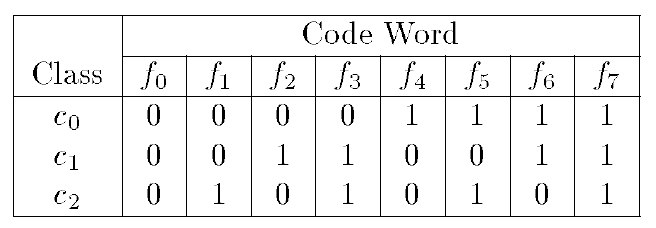
\includegraphics[width=.8\textwidth]{figure/codeword.png} %1.png是图片文件的相对路径
			\caption{3类8位编码} %caption是图片的标题
			\label{img} %此处的label相当于一个图片的专属标志,目的是方便上下文的引用
		\end{figure}
		\item 令码长为8,类别数为4,试给出海明距离意义下的最优ECOC编码,并简述构造思路。
		\item 试简述好的纠错码应该满足什么条件?(请参考完整版阅读资料)
		\item ECOC编码能起到理想纠错作用的重要条件是:在每一位编码上出错的概率相当且独立,试分析多分类任务经ECOC编码后产生的二类分类器满足该条件的可能性及由此产生的影响。
	\end{enumerate}	
	\item \textbf{[10 pts]} 使用OvR和MvM将多分类任务分解为二分类任务求解时,试论述为何无需专门这对类别不平衡进行处理。
\end{enumerate}
\subsection{模型推广}
\textbf{[10 pts]} 对数几率回归是一种简单的求解二分类问题的广义线性模型,试将其推广到多分类问题上,其中标记为$y\in\{1,2\dots,K\}$。

提示:考虑如下$K-1$个对数几率
$$\ln\frac{p(y=1|\mathbf{x})}{p(y=K|\mathbf{x})},	\ln\frac{p(y=2|\mathbf{x})}{p(y=K|\mathbf{x})},\cdots,	\ln\frac{p(y=K-1|\mathbf{x})}{p(y=K|\mathbf{x})}$$

\begin{solution}
	~\\4.1
	\begin{enumerate}[(1)]
		\item 
		OvO的复杂度$\frac{C(C-1)}{2}\mathcal{O}(\frac nc)\times2=\mathcal{O}(Cn)$。\\
		OvR的复杂度$C\mathcal{O}(n)=\mathcal{O}(Cn)$。
		\item 
		\begin{enumerate}[1)]
			\item 
			可以纠正$\lfloor\frac{n}{2}\rfloor$个分类器的错误。
			$c_0$和$c_1$的海明距离为4,$c_1$和$c_2$的海明距离为4,$c_0$和$c_2$的海明距离为4,最小海明距离为4。当两个分类器出错时,某些编码无法纠错,例如00101011,其与$c_0$、$c_1$、$c_2$的海明距离分别为2、2、4。
			\item 
			码长为8,类别数为4,海明距离意义下的最优ECOC编码,第$i$行由$2^{4-i}$个0和$2^{4-i}$个1交替组成。
			\begin{center}
				\begin{tabular}[h]{|*{9}{c|}}
				\hline
				  & 0 & 1 & 2 & 3 & 4 & 5 & 6 & 7\\
				\hline
				0 & 0 & 0 & 0 & 0 & 0 & 0 & 0 & 0 \\
				1 & 0 & 0 & 0 & 0 & 1 & 1 & 1 & 1 \\
				2 & 0 & 0 & 1 & 1 & 0 & 0 & 1 & 1 \\
				3 & 0 & 1 & 0 & 1 & 0 & 1 & 0 & 1 \\
				\hline
				\end{tabular}
			\end{center}
			\item 
			行分离,行之间的海明距离较大。列分离,列之间不相关,即海明距离较大。
			\item 
			满足该条件的概率很低,因为不同类别之间的距离不一样,例如手写数字识别中5比1更“接近”6,所以编码出错概率难以相当,也很难保证独立,这产生的影响是实际误差可能远大于ECOC编码的理论误差。
		\end{enumerate}
	\item 
	因为对每个进行了相同的处理,其拆解出的二分类任务中类别不平衡的影响会相互抵消。
	\end{enumerate}
	4.2\\
	对$K-1$个对数几率使用线性模型
	\[\ln\frac{p(y=i|\mathbf{x})}{p(y=K|\mathbf{x})}=w_i^Tx+b_i,\quad i=1,2,\cdots,K-1\]
	再考虑概率之和为1,得到
	\[
	p(y=i|\mathbf{x})=
	\begin{cases}
	\frac{e^{w_i^Tx+b_i}}{1+\sum_{j=1}^{K-1} e^{w_j^Tx+b_j}}\quad i=1,2,\cdots,K-1\\
	\frac{1}{1+\sum_{j=1}^{K-1} e^{w_j^Tx+b_j}},\quad i=K
	\end{cases}
	\]
\end{solution}
\bibliographystyle{plain}
\bibliography{ref.bib}
\end{document}